\chapter{The Large Hadron Collider}
The Large Hadron Collider (LHC) is a 26.7 km circular high-energy particle accelerator, spanning the Swiss-French border near the city of Geneva, Switzerland \cite{LHC_machine}. The LHC occupies the tunnel constructed in 1989 for the Large Electron-Positron (LEP) Collider, and reaches a maximum depth of 170m below the surface. The LHC is operated by the European Organization for Nuclear Research (CERN), the largest international scientific collaboration in the world.\par

The LHC accelerates protons and heavy ions, and collides them at four interaction points around the ring, with a design center-of-mass energy per collision of $\sqrt{s}$ = 14 TeV. Each interaction point is home to one of four detector experiments, which study the products of the collisions. The largest of these experiments is the ATLAS detector, a general purpose detector designed to study the Standard Model and search for new physics that could be produced in LHC collisions \cite{ATLAS_at_LHC}. The CMS detector is another general purpose detector, designed and operated independently of the ATLAS detector, but intended to probe the same range of physics \cite{CMS_at_LHC}. The ALICE experiment is a dedicated heavy ion experiment, and the LHC-b experiment is a dedicated $b$-physics experiment  \cite{ALICE_at_LHC} \cite{LHCb_at_LHC}.\par

This chapter will cover the multi-component accelerator complex powering the LHC, the state-of-the-art magnets which steer the particle beams, measurements of the intensity and number of collisions produced by the LHC, and finally an overview of LHC activities in the past, present, and future.

 \section{Accelerator Physics}
 \subsection{The Journey of a Proton}
 \label{sec:proton_journey}
From 2010 - 2018, the protons which fed the LHC started as hydrogen gas. The electrons were removed from the hydrogen atoms through the use of strong electric fields. The linear accelerator LINAC2 then accelerated the protons to an energy of 50 MeV. Between 2018 and 2020, LINAC2 was replaced with LINAC4, which instead accelerates $H^{-}$ ions, hydrogen atoms with two electrons. LINAC4 is capable of accelerating the $H^-$ ions to 160 MeV. Before injection to the next part of the acceleration chain, both electrons are stripped from the $H^-$ ions, leaving just protons. From here the protons enter the Proton Synchrotron booster, where they are accelerated up to 1.4 GeV of energy. Subsequently they are sorted into bunches separated in time by 25 ns, where each bunch contains approximately $10^{11}$ protons. Next the bunches pass through the Proton Synchrotron (PS) and the Super Proton Synchrotron (SPS), where they reach energies of 25 GeV and 450 GeV respectively. Finally they are injected into the LHC as two beams traveling in opposite direction. The original design allowed each beam to be accelerated up to 7 TeV of energy. Due to limitations in the performance of the superconducting LHC magnets, the highest energy actually achieved by the LHC beams during Run 2 was 6.5 TeV, giving a collision center-of-mass energy of $\sqrt{s}$ = 13 TeV \cite{lhc_faq}. Figure \ref{fig:accelerator_complex} shows the full LHC accelerator complex.\par

\begin{figure}
	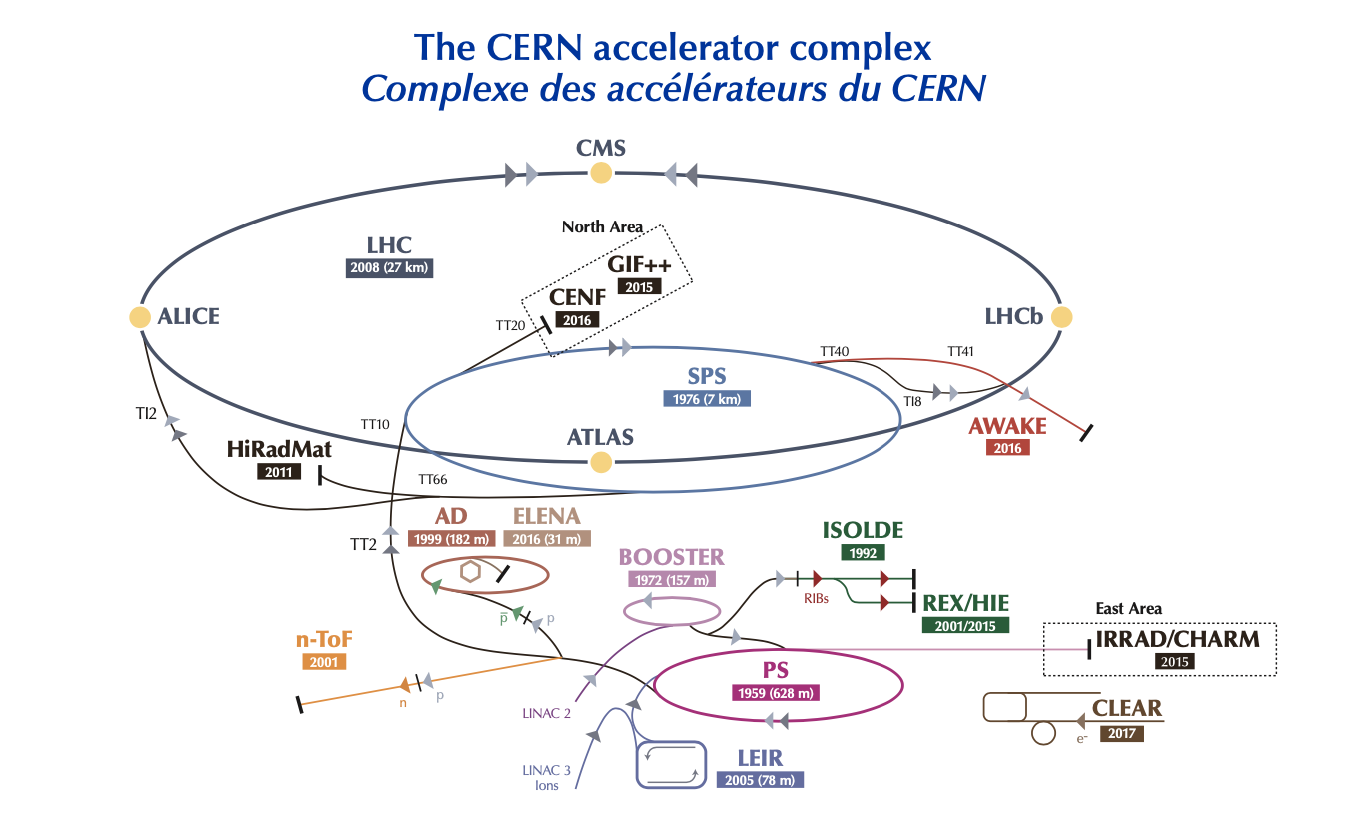
\includegraphics[width=\textwidth]{figures/ch3/accelerator_complex.png}
	\caption{The LHC accelerator complex at CERN \cite{cern_accelerator_complex}}
	\label{fig:accelerator_complex}
\end{figure}

 Acceleration in the LHC is performed by eight radio frequency (RF) cavities located around the ring. Each RF cavity produces a 2 MV electric field oscillating at 40 MHz. The 40MHz oscillation produces a point of stable equilibrium every 2.5 ns. These points of equilibrium are synchronized with the occurrence of the proton bunches produced in the PS -- a proton bunch occupies one out of every ten points of stable equilibrium, such that the bunches maintain a 25 ns spacing \cite{lhc_faq}. \\

\subsection{Magnets}
In addition to the acceleration cavities, the LHC houses 9593 superconducting magnets which direct and focus the proton beam on its 27 kilometer journey. The magnets are comprised of superconducting Niobium-Titanium coils cooled to 1.9K by superfluid helium. As the beams approach one of the four collision points around the ring, multipole magnets focus and squeeze the beam for optimal collisions \cite{lhc_faq}.\par

The LHC is divided into sections, where each section contains an a smoothly curving \textit{arc} and a straight \textit{insertion}. The arcs are composed of 1232 large dipole magnets which bend the beam to follow the roughly circular 27 km path. The main dipoles generate powerful 8.3 tesla magnetic fields to achieve this bend. Each dipole magnet is 15 meters long and weighs 35 tonnes. The dipoles work in conjunction with quadrupole magnets, which keep the particles in a focused beam, and smaller sextupole, octupole and decapole magnets which tune the magnetic field at the ends of the dipole magnets \cite{lhc_magnets}.\par

The straight insertion sections have different purposes depending on their location around the ring: beam collisions, beam injection, beam dumping, or beam cleaning. At the four collision points, insertion magnets squeeze the beam to ensure a highly focused collision. This is accomplished with a triplet of quadrupole magnets, which tighten the beam from 0.2 millimeters to just 16 micrometers in diameter. Insertion magnets also clean the beam, which prevents stray particles from hitting sensitive components throughout the LHC. When the LHC is ready to dispose of a beam of particles, beam dump magnets deflect the path of the beam into a straight line towards a block of concrete and graphite that stops the beam. A dilution magnet then reduces the beam intensity by a factor of 100,000 before the final stop \cite{lhc_magnets}. Figure \ref{fig:lhc_octants} shows the locations various beam activities.\par

\begin{figure}
        \centering
	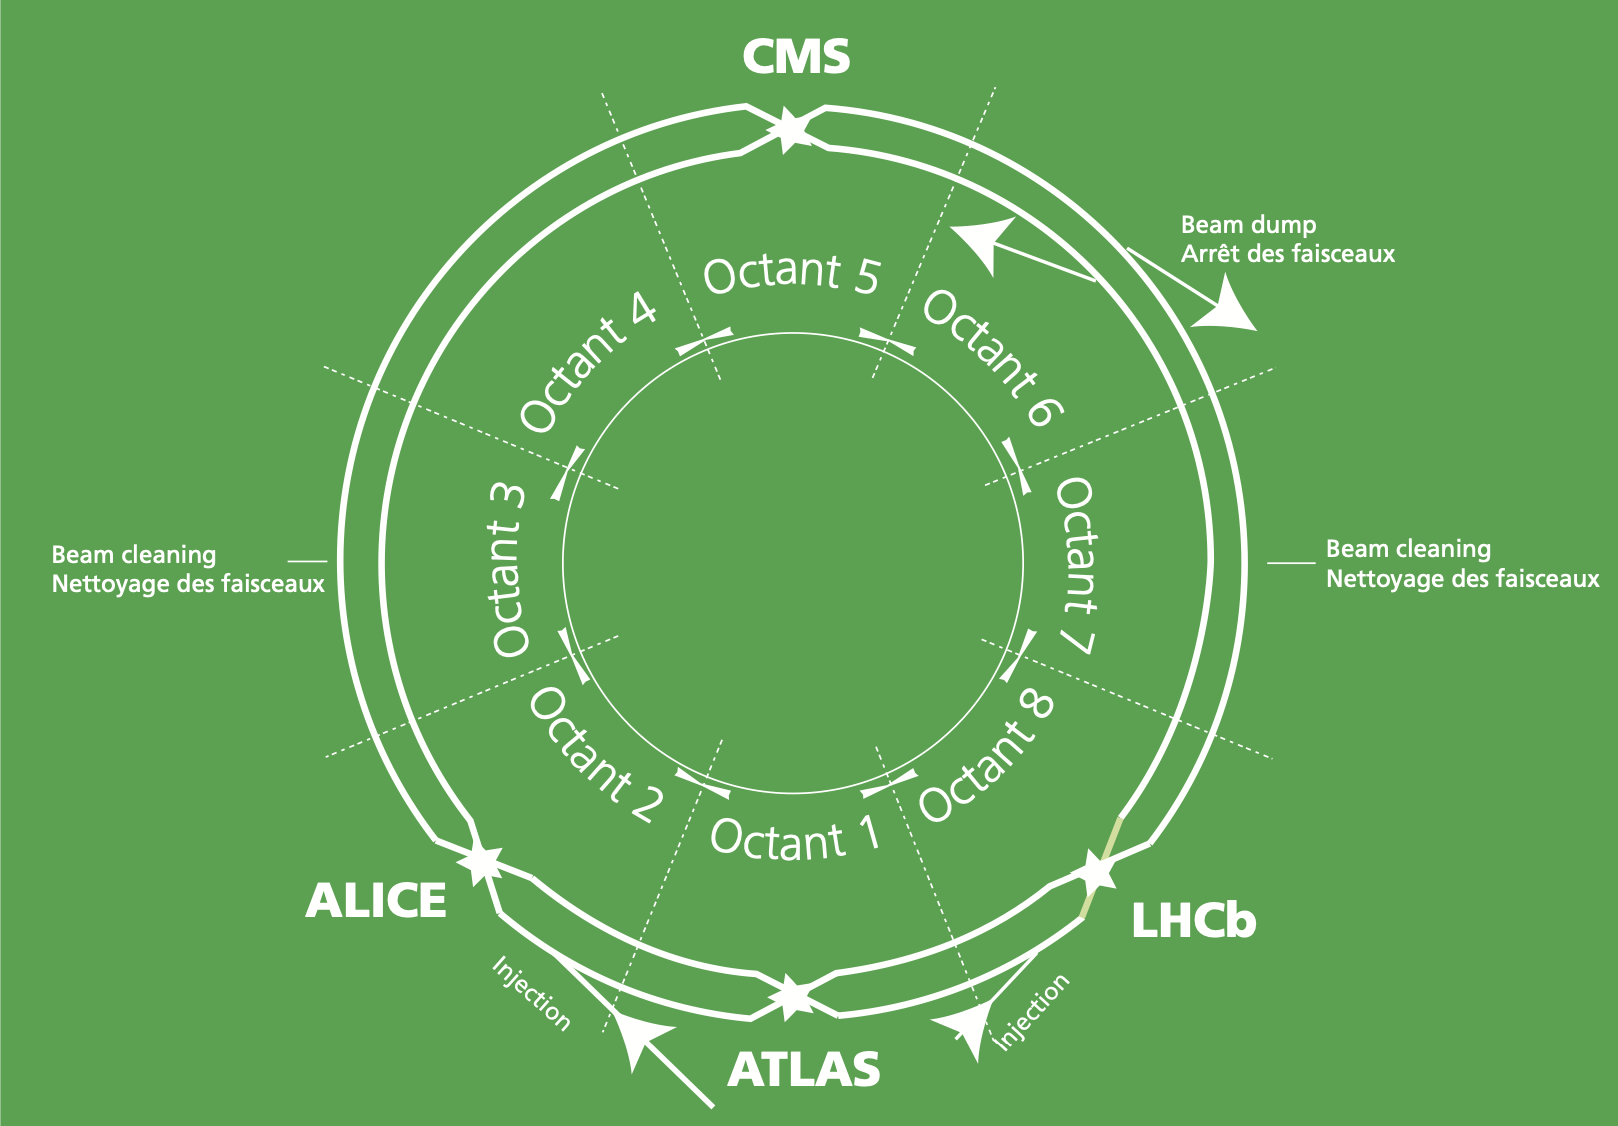
\includegraphics[width=.7\textwidth]{figures/ch3/lhc_octants.png}
	\caption{The octants of the LHC and location of various beam activities \cite{lhc_faq}. Stars indicate the locations of beam collisions, and the associated detectors recording the outcome of those collisions.}
	\label{fig:lhc_octants}
\end{figure} 
 
 \section{Luminosity}
 
Collisions at the LHC occur when the two beams of proton bunches cross at one of the four interaction points. The intensity of collisions is described by the instantaneous luminosity, the formula for which is given in equation \ref{eq:lumi}.  
 \begin{equation}
	L = \frac{f N_1 N_2}{4 \pi \sigma_x \sigma_y}
	\label{eq:lumi}
\end{equation}

Here $f$ is the revolution frequency, $N_1$ and $N_2$ are the number of particle per bunch for each beam, and $\sigma_x$, $\sigma_y$ are the horizontal and vertical beam widths. \par

The instantaneous luminosity gives the number of the collisions that could be produced at the interaction point per unit of cross-sectional area per unit of time, generally expressed in cm\textsuperscript{-2}s\textsuperscript{-1}. The integrated luminosity is obtained by integrating the instantaneous luminosity over a given block of time, and measures the total number of collisions which have occurred during that operation period. The total integrated luminosity is directly correlated with the size of the datasets collected by the LHC experiments. Total integrated luminosity for Run 2 is illustrated in Figure \ref{fig:lumi_run2}. \par 

High levels of instantaneous luminosity result in multiple $pp$ collisions per bunch crossing, which leads to an effect known as $pileup$. Pileup poses a challenge for detector physics, as reconstructing the products of multiple simultaneous events is far more challenging than reconstructing a single event with no pileup. Pileup conditions vary from year-to-year and run-to-run of LHC operation, and the impact of these conditions are taken into account when analyzing the data, as will be discussed further in Chapter \ref{ch:part_reco}. Measurement of pileup conditions during Run 2 are illustrated in Figure \ref{fig:lumi_run2}. \par
 
 \begin{figure}
     \centering
     \begin{subfigure}[b]{0.49\textwidth}
         \centering
         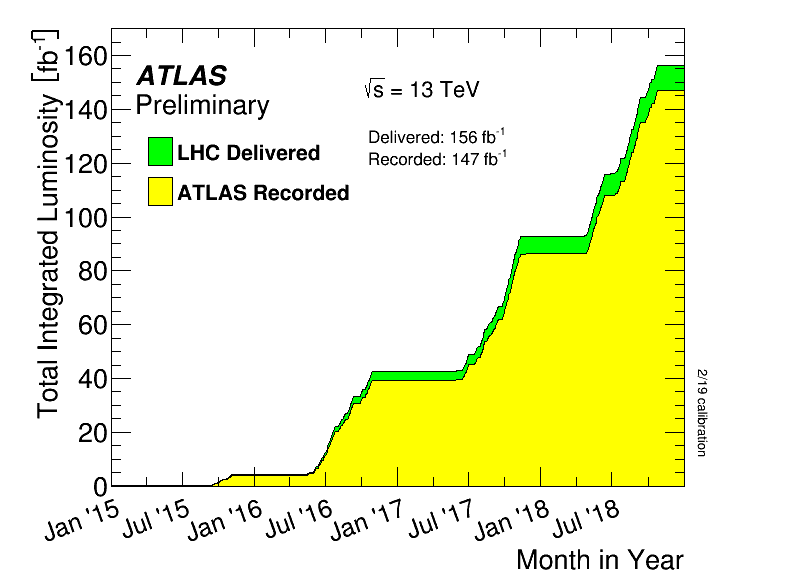
\includegraphics[width=\textwidth]{figures/ch3/lumi_integrated.png}
     \end{subfigure}
     \hfill  
     \begin{subfigure}[b]{0.48\textwidth}
         \centering
         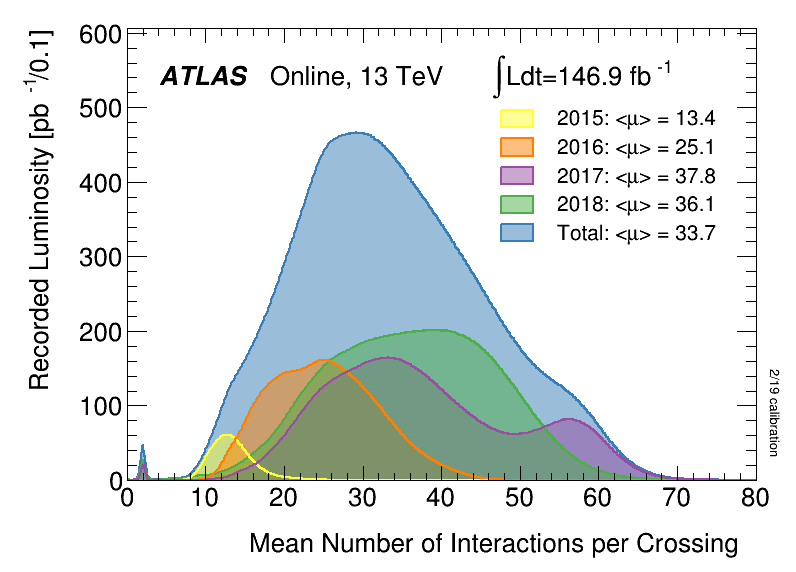
\includegraphics[width=\textwidth]{figures/ch3/lumi_instantaneous.png}
     \end{subfigure}
     \hfill
     \caption { (Left) Total integrated luminosity over the course of Run 2. (Right) Average number of $pp$ interactions per bunch crossing in Run 2. Each curve is weighted by the integrated luminosity for the year.}
     \label{fig:lumi_run2}
\end{figure}
 
 The design peak luminosity of the LHC is $1.0 \times 10^{34}$ cm\textsuperscript{-2}s\textsuperscript{-1}. During Run 1 of the LHC the peak instantaneous luminosity was $0.8 \times 10^{34}$ cm\textsuperscript{-2}s\textsuperscript{-1}. Over the course of Run 1 the LHC collected a total integrated luminosity of 5.46 \invfb at $\sqrt{s} = 7$ TeV, and 22.8 \invfb at $\sqrt{s} = 8$ TeV. Following the first long shutdown and upgrade phase of operations, the LHC achieved a center of mass energy $\sqrt{s} = 13$ TeV at the beginning of Run 2 in 2015. The LHC was also able to deliver $2.0 \times 10^{34}$ cm\textsuperscript{-2}s\textsuperscript{-1} peak instantaneous luminosity, double the design value. During LHC Run 2, from 2015-2018, the LHC delivered 156 \invfb of integrated luminosity for proton-proton collisions. Run 3 of the LHC began in 2022, and is expected to deliver $250$ \invfb of integrated luminosity to the ATLAS and CMS experiments by 2026 \cite{lhc_timeline}.\par
 
The goal of LHC physic analyses is to find and study rare events produced by interesting physics processes. The cross section $\sigma$ of a given process indicates the probability of that process occurring given the beam conditions of the LHC. Multiplying the cross section by the integrated luminosity of a dataset gives the expected number of events for that process within the dataset.

 \begin{equation}
	N\textsubscript{events} = \int \sigma L(t) dt = \mathcal{L} \times \sigma
	\label{eq:xs}
\end{equation}

The cross section for most processes of interest, especially BSM processes, is several orders of magnitude below the total cross section for the LHC. Therefore maximizing the number of events produced in collisions is crucial to increase the likelihood of producing events from processes of interest. For this reason, maximizing instantaneous luminosity is a key factor in accelerator design and operation, while mitigating the resulting pileup effects is a key component in detector design and operation. \par 

\section{LHC Timeline}
The first proton-proton collisions at the LHC were achieved in 2010 with a center-of-mass energy of $\sqrt{s}$ = 7 TeV. Run 1 of the LHC took place between 2010 and early 2013, during which time the center-of-mass collision energy increased from 7 TeV to 8 TeV. Figure \ref{fig:lhc_timeline} shows an overview of LHC activities beginning in 2011, in the midst of Run 1. The data collected during Run 1 led to the discovery of the Higgs Boston in 2012 \cite{higgs_paper}. \par

Between 2013 and 2015 the LHC underwent the first Long Shutdown (LS1) during which time maintenance and renovation was performed on the accelerator chain, including the repair and consolidation of the high-current splices which connect the super-conducting LHC magnets. Run 2 of the LHC took place from 2015 to 2018 and achieved a center-of-mass energy of $\sqrt{s}$ = 13 TeV. Analysis of data collected in Run 2 is still on going, and is the subject of study in this thesis. \par

Between 2018 and 2022 the LHC underwent the second Long Shutdown (LS2), allowing for further detector and accelerator maintenance and upgrades. Key improvements to the LHC included the improvement of the insulation for over 1200 diode magnets, and the upgrade from LINAC2 to LINAC4 mentioned in Section \ref{sec:proton_journey}. Run 3 of the LHC began in 2022 and achieved a center-of-mass energy of $\sqrt{s}$ = 13.6 TeV. \par

Run 3 is scheduled to continue through 2026, at which point the LHC machine and detectors will undergo upgrades for the \textit{high luminosity} LHC (HL-LHC). The HL-LHC will increase the instantaneous machine luminosity by a factor of 5 - 7.5 with respect to the nominal LHC design. The bottom panel of Figure \ref{fig:lhc_timeline} shows an overview of the preparation work for the HL-LHC that has been going on concurrently with Run 1, 2, and 3 of the LHC \cite{hl_lhc}. 

\begin{figure}
        \centering
	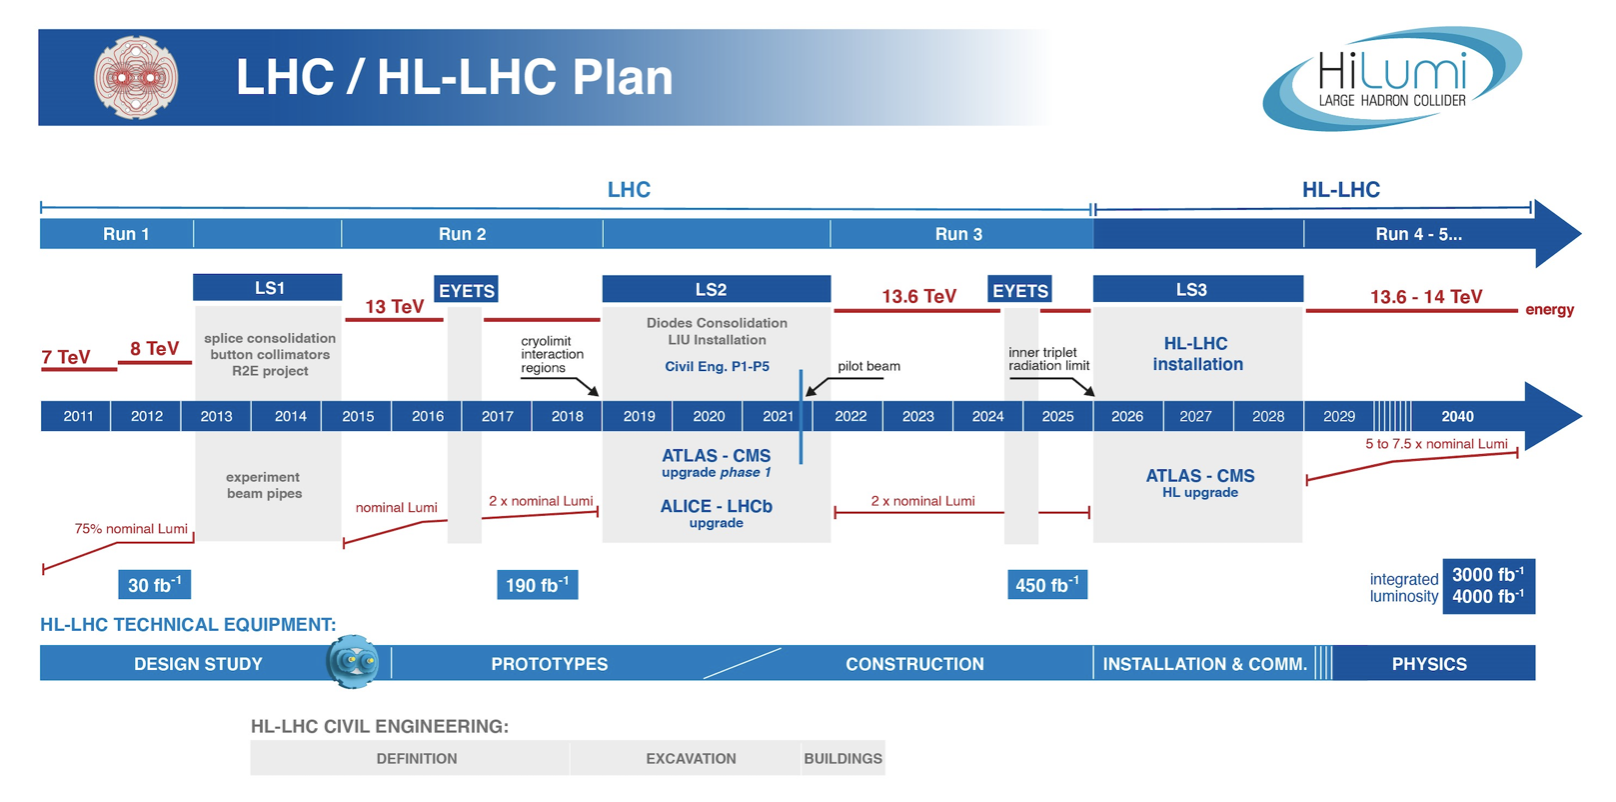
\includegraphics[width=0.9\textwidth]{figures/ch3/hl_lhc_timeline.png}
	\caption{Timeline of LHC and HL-LHC activities \cite{lhc_timeline}. Integrated luminosity estimates are approximate, and not reflective of the exact amount delivered to each experiment.}
	\label{fig:lhc_timeline}
\end{figure}
